\documentclass[cs4size]{ctexartutf8} 
\usepackage[unicode={true}]{hyperref}
\hypersetup{colorlinks,%
                 citecolor=black,%
                 filecolor=black,%
                 linkcolor=black,%
                 urlcolor=blue,%
                 pdftex}

\usepackage{graphicx}
\usepackage{float}

				
\author{YXY}
\title{脸脸应用设计方案}

\begin{document} 

\maketitle
\tableofcontents

\section{脸脸网站}
脸脸的官方网站是\href{http://www.dface.cn}{http://www.dface.cn}。官方网站的用途是提供脸脸手机应用的介绍、下载和反馈。个人用户无法利用网站登录和使用脸脸,商家可以通过网站登录到商家管理后台。


脸脸网站的设计可以参考微信官方网站,主要提供“首页 ,下载 , 最新消息,常见问题,商家加盟,联系我们”等几个栏目。总体上来说比较简单。


注意:目前官方网站的phone目录下是手机应用的原型设计,但是网站上线后,phone目录会禁止访问。phone目录下的文件也禁止引用网站其它部分的文件。


\section{手机端应用}
手机端应用的设计主要参照现有的原型设计。这里只是补充原型设计里无法描述的其它信息。

\subsection{登录}

\begin{figure}[H]
\centering

\includegraphics[scale=0.5]{./1.png}
\label{p1}
\end{figure}

登录界面中目前只有新浪微博登录一种方式,以后会考虑添加腾讯微博等其它的登录方式。当用户量达到一定规模,首页可以增加一些总的统计数字:如总共有多少人摇了一摇等。

\subsection{上传照片}

\begin{figure}[H]
\centering

\includegraphics[scale=0.5]{./2.png}
\end{figure}

上传照片时要以异步的方式在后台上传,不影响用户点完成。在此页面,附近的脸提供静态的虚拟脸即可,以刺激用户上传头像。当应用达到一定规模后,提供动态的附近的受欢迎的头像。

\subsection{现场}

\begin{figure}[H]
\centering

\includegraphics[scale=0.5]{./3.png}
\end{figure}

“现场”是用户登录后的首页,如果用户没有主动退出登录,那么每次重新打开脸脸后都直接进入“现场”。

“现场”所显示的商家是需要根据经纬度计算出来的,会有时间延迟和距离误差。时间延迟在2秒到30秒左右,价格便宜的手机往往会迟延时间长。经纬度的距离误差在10米到1000米左右。多次测量,经纬度的距离误差会越来越小。

因为获取现场有时间延迟,所以在还未获得现场时,现场名称栏要显示转动的图标。获取现场成功后,图标停止。

因为经纬度有距离误差,所以现场的计算结果很可能不是用户真正的现场。因此用户需要能够手动选择目前所在的现场。

此外,有些商家本身就距离很紧,比如南山路的酒吧。此时用经纬度无法准确定位。因此客户端要判断从服务器获得的前三个商家之间本身的距离是否少于20米,如果小于这个数字,直接让用户选择商家,而不是默认给出一个商家作为现场。

因为经纬度的距离误差可以获取,如何以直观的方式告诉用户当前现场的准确度?比如百度地图以圈圈的方式显示当前位置的精确度,圈越小越精确。



用户确认了自己的现场后,在同一次使用范围内(应用未退出)不再计算现场。但是当用户切换到其它应用后再次使用脸脸,此时根据当前新的经纬度确定是否重新计算。当新的地点和原地点相差1000米以上时,需要重新计算获取现场。

现场附近的用户的获取也需要时间,所以当附近用户的图像还未获取时,如何处理?是显示上次现场附近的脸,还是系统默认的一组脸?

\subsection{关于摇一摇}
在现场摇一摇以后,就进入现场的群聊页面。摇一摇有多个功能,包括:给现场的所有人打招呼;在现场签到和确认当前的现场;如果商家有抽奖等活动,参与抽奖。

此外,在进入群聊页面后也可以摇一摇。此时的含义是参与商家发起的活动。


\subsection{现场群聊}

\begin{figure}[H]
\centering
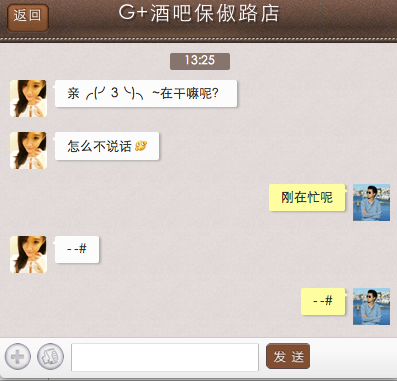
\includegraphics[scale=0.5]{./4.png}
\end{figure}

商家可以申请帐户绑定功能,将个人帐户与商家帐户绑定。比如商家的老板用自己的手机登录脸脸。此时,他登录脸脸后的发言会有单独的醒目的样式。商家帐户不能登录使用脸脸手机应用,只能登录脸脸网的商家管理后台。一个商家帐户可以绑定多个个人帐户。个人帐户采用新浪微博认证,商家帐户由脸脸网建立和管理。

现场群聊要给商家预留一行发布公告的地方。如果商家没有公告,此行自动隐藏。商家公告目前要在网站商家后台管理,以后考虑可以直接通过手机管理。

商家公告一般发布一些重要的、实效性在一天以上的信息。一些临时的信息可以在群聊页面用手机直接发布。


商家可以在群聊页面发起活动。比如主持人喊一二三,大家摇手机,摇到前10名的有奖。具体的活动规则由商家自行拟定。用户领奖时发一个确认信息给发起人即可。


\subsection{附近}

\begin{figure}[H]
\centering
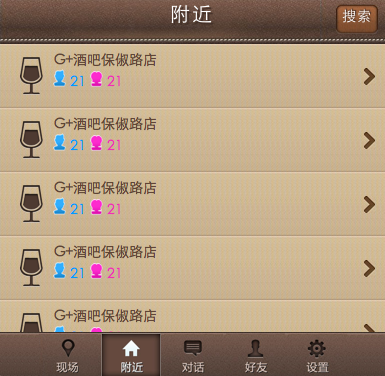
\includegraphics[scale=0.5]{./5.png}
\end{figure}

附近的商家默认按距离由近到远排序,要能按类别(酒吧、餐饮、活动等)筛选,按名称查询等。

附近的商家如果和用户当前的距离在1000米以内,可以进入该商家的现场,参与活动和发言。如果超过1000米,该用户只能查看该商家的信息。

附近的商家应该支持下拉获取更多数据功能和上拉刷新功能。所以类似的列表也都应该支持下拉和上拉操作。

如果是用户只能查看该商家,其界面如何设计?


\subsection{对话}

\begin{figure}[H]
\centering

\includegraphics[scale=0.5]{./6.png}
\end{figure}

对话应该包括两种类型:一种是个人之间的对话,一种是个人和组织的对话。两种对话要有不同的显示样式。个人在商家现场的群聊以及商家发送的信息以商家名义出现在会话中。系统通知消息应该出现在“脸脸”系统用户中。中奖消息应该以商家的名义发出还是“脸脸”的名义发出?


\subsection{个人聊天}

\begin{figure}[H]
\centering

\includegraphics[scale=0.5]{./7.png}
\end{figure}

个人聊天页面类似于群聊页面。其中聊天时支持的表情和动作还需要细化。点击摇一摇图标时,进入一个专门的摇一摇的界面,和微信类似。比如摇一摇的体验包括:动作 – 摇动;视觉 – 屏幕裂开并合上来响应动作; 听觉:有吸引力(男性是来福枪,女性是铃铛)的声音来响应动作;结果是发送一个消息。



\subsection{好友}

\begin{figure}[H]
\centering
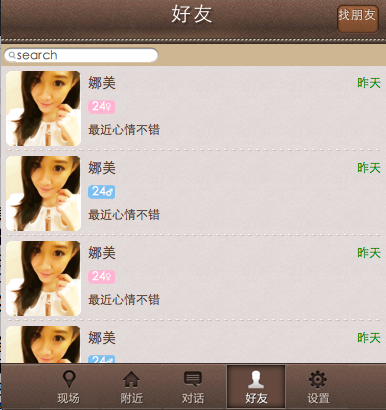
\includegraphics[scale=0.5]{./8.png}
\end{figure}

这里的好友是用户在脸脸上加的好友,且是单向关系(无需对方确认),和新浪微博没有关系。

找朋友目前要支持手机通讯录和从新浪微博好友两种来源。对于对方未加入脸脸的,可以发送邀请;对于已加入脸脸的,可以直接发送消息。

\subsection{个人信息}

\begin{figure}[H]
\centering
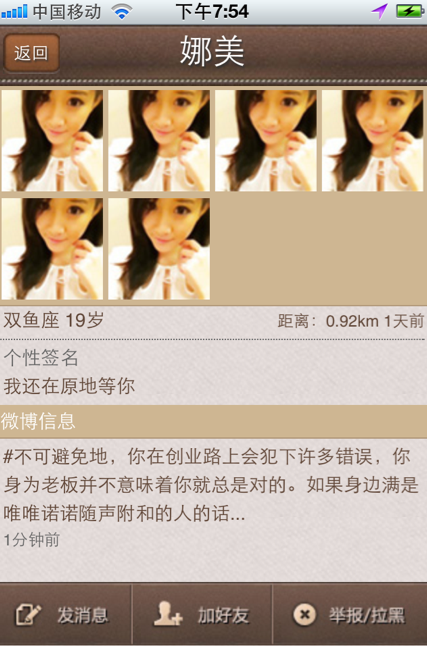
\includegraphics[scale=0.5]{./9.png}
\end{figure}

个人信息中的图片取自用户新浪微博中发的微博中的图片。距离改成地点。

\subsection{设置}

\begin{figure}[H]
\centering
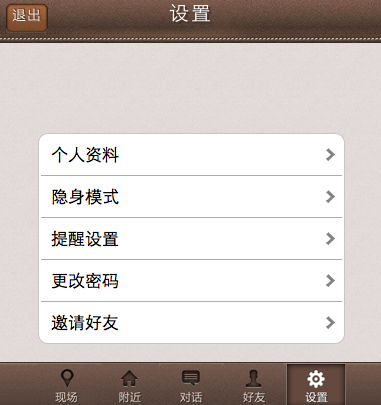
\includegraphics[scale=0.5]{./10.png}
\end{figure}

设置页面中,在菜单中要增加“退出”的功能,同时取消“修改密码”功能。“提醒设置”的功能要明确。有两种提醒,一种是系统消息,一种是好友在附近时的提醒。这两种提醒的实现机制不一样。系统消息采用应用内通知即可。好友在附近时的提醒最好是Push提醒,这样用户没使用脸脸时也能收到提醒。



\section{脸脸网商家后台管理功能}
\subsection{商家帐户登录}
只有认证过的商家才能登录。认证后给商家提供登录名和密码。

\subsection{关联个人帐户}
商家可以自行关联多个个人帐户。关联后的个人帐户可以以商家的身份在脸脸应用中发言。目前只提供关联一个帐户的能力。

\subsection{管理滚动广告}
商家可以管理现场群聊页顶部的滚动广告。给商家提供最多3条滚动广告发布的权限。


\subsection{抽奖管理}
如何运营?


\section{脸脸网管理员后台管理功能}
商家信息获取和管理、商家帐户认证、权限管理、运营需要的支撑功能等。

待细化。



\section{脸脸网服务器与手机端的开发接口}
\subsection{用户注册}
脸脸应用直接使用新浪微博的用户系统,所以从用户的角度看不需要主动在脸脸中注册。但是为了统计当前登录的用户信息,管理用户的聊天信息和好友关系,必须建立自己的用户系统。

用户注册的逻辑是:当手机用户经过新浪认证后,给脸脸网服务器发送登录成功的消息。服务器端判断该用户是否是首次使用脸脸,如果是首次使用,那么自动创建用户系统。

\subsection{用户登录}
手机用户经过新浪认证登录后,要在回调函数中通知脸脸网该用户登录了。
如果采用Xauth,登录成功后调用下面的链接(目前采用http协议,正式版会采用https协议)。



\begin{table}[H]
   \begin{center}
\begin{tabular}{|c|p{12cm}|}
\hline
\multicolumn{2}{|c|}{http://www.dface.cn/user/login} \\
\hline\hline
 \  参数  &  说明  \\
\hline
 username  &  用户名\\
\hline
 password  &  微博密码\\ 
\hline
 hash  &  hash码,采用SHA-1算法并取前16位。
 
  待hash串为:username+password+AppKey+AppSecret+date
  
  \\
\hline
\end{tabular}
\caption{用户登录接口}\label{tab0}
   \end{center}
\end{table}


其中,AppKey和AppSecret为脸脸网在新浪微博的key和secret,分别为:

AppKey: "2054816412"

AppSecret: "75487227b4ada206214904bb7ecc2ae1"
  

HASH的计算例子:
比如用户名“name”,密码“123456”,当前日期“2012-05-18”,那么待hash字符串为“name123456205481641275487227b4ada206214904bb7
ecc2ae12012-05-18”。hash后的值为 " 833660667c6d9c3a "。

ruby计算代码为:
Digest::SHA1.hexdigest(str)[0,16]



服务器的返回结果为json串,格式为:
\{code : 1, user\_id: 123, desc: "name登录成功"\}

其中,code的可能取值为:1登录成功,2重复登录,3Hash不匹配,4其它错误。user\_id表示该用户在脸脸网的id。




\subsection{用户退出}
手机用户退出时要先调用新浪的退出,然后通知脸脸网该用户退出了。

\begin{table}[H]
   \begin{center}
\begin{tabular}{|c|p{12cm}|}
\hline
\multicolumn{2}{|c|}{http://www.dface.cn/user/logout} \\
\hline\hline
 \  参数  &  说明  \\
\hline
 username  &  用户名\\
\hline
 password  &  微博密码\\ 
\hline
 hash  &  同上\\
\hline
\end{tabular}
\caption{用户退出接口}
   \end{center}
\end{table}


\subsection{上传个人头像}

\begin{table}[H]
   \begin{center}
\begin{tabular}{|c|p{12cm}|}
\hline
\multicolumn{2}{|c|}{http://www.dface.cn/user/\#\{user\_id\}/user\_logos} \\
\hline\hline
 \  参数  &  说明  \\
\hline
 user\_logo[uploaded\_data]  &  上传的文件\\
\hline
 lng  &  纬度\\ 
\hline
\end{tabular}
\caption{上传个人头像}
   \end{center}
\end{table}

请求必须用POST方式提交,并且注意采用multipart/form-data编码方式

enctype="multipart/form-data" method="post"

\subsection{设置个人信息}
\begin{table}[H]
   \begin{center}
\begin{tabular}{|c|p{12cm}|}
\hline
\multicolumn{2}{|c|}{http://www.dface.cn/user\_info} \\
\hline\hline
 \  参数  &  说明  \\
\hline
 user\_id  &  用户id\\
\hline
 ...  &  \\ 
\hline
\end{tabular}
\caption{设置个人信息}
   \end{center}
\end{table}

请求必须用POST方式提交。

\subsection{获得个人信息}
\begin{table}[H]
   \begin{center}
\begin{tabular}{|c|p{12cm}|}
\hline
\multicolumn{2}{|c|}{http://www.dface.cn/user\_info} \\
\hline\hline
 \  参数  &  说明  \\
\hline
 user\_id  &  用户id\\
\hline
\end{tabular}
\caption{设置个人信息}
   \end{center}
\end{table}



\subsection{根据经纬度获得附近的商家}

\begin{table}[H]
   \begin{center}
\begin{tabular}{|c|p{12cm}|}
\hline
\multicolumn{2}{|c|}{http://www.dface.cn/mshop/aroundme} \\
\hline\hline
 \  参数  &  说明  \\
\hline
 lat  &  经度\\
\hline
 lng  &  纬度\\ 
\hline
\end{tabular}
\caption{根据经纬度获得附近的商家}
   \end{center}
\end{table}



\subsection{根据经纬度获得附近的用户}
本条目及以下部分待细化

\subsection{获取给定商家的信息}


\subsection{获得登录用户的好友信息}

\subsection{获得登录用户的会话信息}

\subsection{添加好友}

\subsection{向给定用户发送信息}

lianlian用户系统和openfire用户系统如何整合,如何sso。
ofUser
聊天室和商家如何整合。
ofMucService
ofMucRoom

自己管理头像还是使用 (vCard-Based Avatars 目前广泛采用)?应该自己管理。

不需要成为好友就可以聊天。不需要roster好友管理功能。脸脸的好友是单向的。

状态: XMPP presence,只有online-offline,没有away,busy等其它状态。

切换应用后,不需要offline,只有用户手动退出时,才主动offline。
服务器端保持online是否消耗资源。如果保持online,但是客户端其实不可用,这时候是否会有消息丢失。

商家聊天室采用MUC方案,进入商家群聊页面就加入room,切换到其它页面时不主动退出,只有当主动加入另一个商家才从当前商家退出。用户永远处在唯一的一个room中。

因为不主动offline,不主动从room退出,如何计算当前room的用户数量?

聊天历史记录功能是否有?
http://community.igniterealtime.org/message/219002#219002
安装Monitoring Service 插件,然后保存在


新加入用户是否可以看到聊天室的历史信息?

聊天室的三种用户,主持者   参与者   访客, 聊天室管理。
黑名单管理。

可靠性。一条信息publish了客户是否能收到了,进一步处理比如说保存或重发等业务逻辑。

Presence处理是IM Server的核心,也是一个IM Server最复杂的部分。一个用户的状态发生变化,需要通过服务器自动投递给他所有在线的好友。openfire是否是自动投送,lianlian是否需要自动投送的能力?



ofPubsubNode什么用途?



\newpage


\end{document}
